%!TEX root = ../thesis.tex
%*******************************************************************************
%****************************** Third Chapter **********************************
%*******************************************************************************
\chapter{Data Description}%Make this title more interesting
In this chapter we will see an overview of the starting data used in this research, as well as some general statistics about it.

\section{Where the data comes from}
The data are tweets collected from the twitter api containing the hashtag \#cop2x with x = [1,2,6], so for each COP we have all the tweets containing the relative hashtag.
For each cop we have two jsonlines files, one for the tweets and one for the users involved. The fields are the one stated in the documentation \footnote{ \href{https://developer.twitter.com/en/docs/twitter-api/data-dictionary/object-model/tweet}{https://developer.twitter.com/en/docs/twitter-api/data-dictionary/object-model/tweet}}, there are many fields but the relevant ones are the following: 

\begin{table}[H]
\centering
\begin{tabular}{|l|l|}
\hline
\textbf{Field} & \textbf{Description} \\ \hline
author & The ID of the author \\ \hline
author\_name & The username of the author \\ \hline
text & The text of the tweet \\ \hline
date & The creation date of the tweet \\ \hline
lang & The language of the tweet \\ \hline
conversation\_id & The ID of the conversation the tweet belongs to \\ \hline
referenced\_type & The type of the referenced tweet \\ \hline
referenced\_id & The ID of the referenced tweet \\ \hline
mentions\_name & The usernames of the mentioned users in the tweet \\ \hline
mentions\_id & The IDs of the mentioned users in the tweet \\ \hline

\end{tabular}
\caption{Description of the fields used of the tweets data}
\label{tab:my_label}
\end{table}
While we use the user's file to map the id of the users to their username, even though not always we have this information, in that case we use the user id as username

\section{Some statistics}
We have data from 3 cops: COP21, COP22, COP26.

\begin{table}[h]
\centering
\setlength{\tabcolsep}{10pt} % Sets the horizontal padding
\renewcommand{\arraystretch}{1.5} % Sets the vertical padding
\begin{tabular}{
  |l|
  S[table-format=7.0,group-four-digits=true]|
  S[table-format=7.0,group-four-digits=true]|
  S[table-format=7.0,group-four-digits=true]|
  S[table-format=7.0,group-four-digits=true]|
}
\hline
 & {\textbf{n\_tweets}} & {\textbf{n\_retweets}} & {\textbf{n\_original}} & {\textbf{n\_original\_with\_retweets}} \\ \hline
\textbf{COP21} & 975040 & 562946 & 412094 & 138427 \\ \hline
\textbf{COP22} & 143278 & 20562 & 63855 & 20562 \\ \hline
\textbf{COP26} & 1558968 & 1191813 & 367155 & 130138 \\ \hline
\end{tabular}
\caption{Dataset Statistics}
\label{tab:my_label}
\end{table}




in fig \ref{fig:cop26_tweets_stats} we can see how the 1'558'968 are distributed, in fact 76\% of them are retweets generated by only 130k original tweets. It is also worth nothing that almost 2/3 of the original tweets have 0 retweets 

\begin{figure}
    \centering
    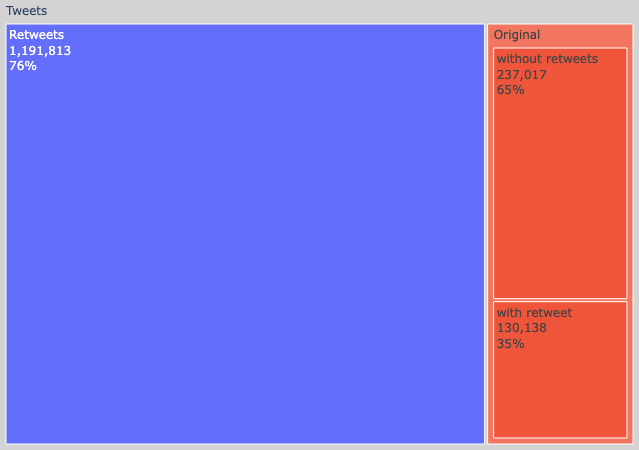
\includegraphics[width=0.9\linewidth]{Chapter3/figures/treemap_tweets-1.png}
    \caption{tweets of cop26}
    \label{fig:cop26_tweets_stats}
\end{figure}








% **************************** Define Graphics Path **************************
\ifpdf
    \graphicspath{{Chapter3/Figs/Raster/}{Chapter3/Figs/PDF/}{Chapter3/Figs/}}
\else
    \graphicspath{{Chapter3/Figs/Vector/}{Chapter3/Figs/}}
\fi

